Tato kapitola pojednává o problematice rozmístění produktů do lokací, anglicky zvané \emph{Storage Location Assignment Problem}, dále pouze zkratka SLAP. V odborné literatuře se lze však setkat s různými variacemi označeními této problematiky, avšak se stejným významem (např.: \emph{Storage Assignment}, \emph{Product allocation/location}, \emph{Slotting}, a~tak dále). Při studiu této problematiky jsem vycházel~z~\cite{slapSeacomp, optimisationOrderPickingGA, exactTimeSlap, whModelSim, slapReview, slapGaMultiObj, slapPickAndPass}.


%%%%%%%%%%%%%%%%%%%%%%%%%%%%%%%%%%%%%%%%%%%%%%%%%%%%%%%%%%%%%%%%%%%%%%%%%%%%%%%%%%%%%%%%%%%


\section{Motivace pro efektivní optimalizaci skladu} % nebo Motivace pro řešení SLAP
\label{motivace}
Sklady slouží pro dočasné uložení produktů (typicky z produkce), které jsou následně postupně získávány za účelem vyřízení zákaznických objednávek. \uv{Pickování} zákaznických objednávek je proces při kterém jsou takto uložené produkty systematicky hledány a přemisťovány z úložných prostor (přesněji slotů lokací), ve kterých jsou dočasně uloženy, do kartonů, ve kterých jsou následně odeslány k zákazníkům. Zákaznické objednávky typicky sestávají z jednotlivých položek, anglicky zvaných \emph{order line}, vždy představující jeden produkt (v anglické literatuře často označován jako \emph{article}, \emph{product}, \emph{code} či \emph{stock keeping unit}) a jeho požadovanou kvantitu (množství). Způsob organizace produktů a jejich pickování značně ovlivňuje výkonnost celého skladu a tedy ovlivňuje efektivnost celého dodavatelského řetězce. To znamená, že čím rychleji budou produkty napickovány, tím rychleji se zákaznická objednávka vyřídí~\cite{optimisationOrderPickingGA}.

Pickování objednávek je jedna z časově nejnáročnějších operací prováděných ve skladu a~je spojena s $55\%$ celkových nákladů skladu, a proto se tedy dle vědců jeví jako nejvhodnější oblast pro optimalizace skladu~\cite{optimisationOrderPickingGA}.

\addtocounter{footnote}{-1}

\begin{figure}[t]
    \centering
    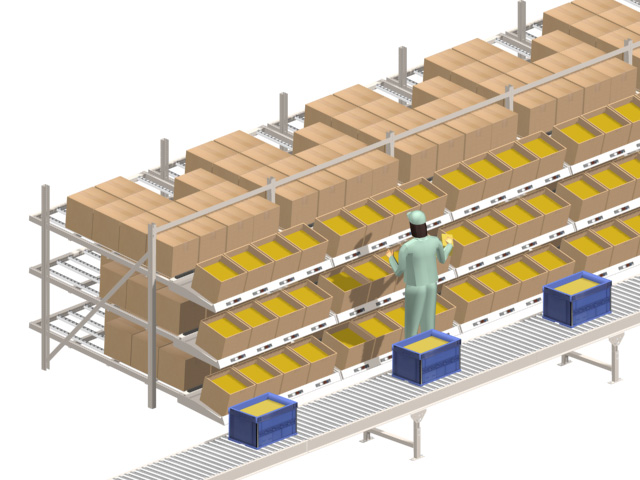
\includegraphics[width=0.8\linewidth]{figures/slap_ea/location_rack.jpg}
    \caption{Příklad pickování objednávek pro vysvětlení terminologie\protect\footnotemark{}. Na obrázku lze vidět lokaci a pickera (pracovník skladu, který vytahuje produkty ze slotů lokace do kartonů objednávek). Způsob fungování je následující: po dopravníku přijede karton, který reprezentuje nějakou objednávku. Uživatel tento karton naskenuje. Systém následně zjistí, které produkty tato objednávka potřebuje, a ukazuje uživateli které produkty (z jakých slotů) má do tohoto kartonu vkládat. Po každém vložení produktu do kartonu uživatel tuto akci potvrdí a pokračuje dalším produktem. Až nasbírá všechny produkty, které jsou na této lokaci potřeba napickovat, systém uživateli řekne, ať karton vloží na dopravník (odkud pokračuje dál), a aby naskenoval další karton, u kterého bude postupovat podobným způsobem.}
    \label{fig:locationRackExplained}
\end{figure}

Proces průmyslové automatizace způsobil požadavky na automatizované skladové systémy v mnoha různých odvětvích. Typické činnosti v takovýchto skladech jsou: příjem zákaznických objednávek a jejich seskupování, třídění a plánování v závislosti na aktuálním množství jednotlivých produktů ve skladu, postupné spouštění objednávek a jejich pickování, až po proces odesílání ze skladu k zákazníkům. Proces pickování objednávek sestává z~několika částí, které značně závisí na typu skladu, jeho komplexitě a v neposlední řadě na použitém informačním systému. Příklad takového pickování společně s popisem terminologie lze vidět na snímku \ref{fig:locationRackExplained}~\cite{whModelSim, optimisationOrderPickingGA}. 

Z pohledu složitosti se SLAP klasifikuje jako NP-těžký problém, a to vzhledem k množství variací způsobených množstvím produktů a úložných prostor. Vzhledem k tomu, mnoho meta-heuristických a heuristických metod bylo použito za účelem řešení této problematiky. Pokud je počet produktů roven počtu úložných prostor, jedná se o problém QAP\footnotemark{}. Pokud počet produktů převyšuje počet úložných prostor, jedná se o problém Knappsack~\cite{slapReview}.

Strategie uložení produktů hraje důležitou roli z pohledu skladových informačních systémů (ang. \emph{warehouse management system}). Tato operace je mnohdy mylně považována za snadnou, ale ve skutečnosti kvůli nejistotě požadavků, variabilitě druhů produktů a potřebě okamžité reakce na změnu na trhu je velmi komplexní a vyžaduje složitá rozhodnutí. Je nutné, aby sklady byly navrženy a řízeny tak, aby byly nákladově efektivní. Náklady na fungování skladu jsou do značné míry určovány již ve fázi návrhu a proto je vhodné před samotnou stavbou skladu věnovat značnou pozornost studiu a analýze budoucího skladu pro dosažení co nejoptimálnějšího skladu pro daný \emph{use-case} (česky případ užití)~\cite{slapSeacomp, slapReview}.

\addtocounter{footnote}{-1}

\footnotetext{Obrázek převzat z \url{http://orderpickingfastfetch.blogspot.com/2013/01/what-is-pick-to-light-pick-to-light-or.html}.}

\stepcounter{footnote}
\footnotetext{QAP -- \emph{Quadratic assignment problem} -- česky problematika kvadratického rozřazení.}

Problematika rozmístění produktů do úložných lokací ve skladu se snaží o nalezení co nejefektivnějšího rozřazení jednotlivých produktů do lokací ve skladu za účelem snížení doby potřebné k vyřízení zákaznických objednávek. To následně velmi ovlivňuje KPI\footnote{KPI -- \emph{Key performance indicators} -- česky výkonnostní klíčové indikátory}~\cite{slapPickAndPass}.

\section{Strategie uložení produktů}
Vzhledem k variabilitě parametrů produktů, které mohou být ve skladu ukládány, existují různé strategie (někdy také zvané jako politiky) uložení produktů do úložných prostor skladu. Při použití skladového informačního systému se tyto možnosti ještě rozšiřují, protože informační systém umožňuje značně větší kontrolu nad celým skladem. Základní strategie pro ukládání produktů jsou následující~\cite{slapSeacomp}\cite{slapPickAndPass}:

\begin{itemize}
    \item \emph{\textbf{Fixed slot}} politika -- Každý slot každé lokace skladu má pevně přiřazený produkt, který obsahuje. Toto nastavení je neměnné. Pro tuto politiku není třeba žádný informační systém a je nejvhodnější z pohledu optimalizací (použito v této práci).
    \item \emph{\textbf{Random}} politika -- Jak z jména vyplývá, produkty jsou rozřazeny do slotů náhodně, což z této politiky dělá jednu z nejlehčích metod. Je velmi rozšířená, protože často vyžaduje méně místa než ostatní metody a umožňuje efektivnější využití úložných prostor. Je také často použita pro srovnání při vyhodnocování výkonnosti ostatních politik.
    \item \emph{\textbf{Frequency-based} politika} -- Přiřazuje nejčastěji pickované/kupované produktu do slotů, které jsou nejblíže ke vstupu a výstupu ze skladu, za účelem sínížení celkové doby zpracování objednávek (použito v této práci pro porovnání).
    \item \emph{\textbf{Class-based} politika} -- Je kompromis mezi jednoduchostí náhodné politiky a přesností (komplexností) politiky založené na frekvenci pickování.
\end{itemize}

Toto je výčet pouze základních politik pro ukládání produktů. Tyto politiky lze mezi sebou dále kombinovat a vytvářet tak složitější, ale účinnější politiky.


\section{Nástroje pro optimalizaci skladu}
Při studiu této podkapitoly jsem vycházel z práce \cite{slapSeacomp}. Nástroj pro optimalizaci skladu by měl být schopen plnit tyto úlohy:

\begin{itemize}
    \item Vytvoření modelu skladu -- Tj. pozice vstupů, výstupů, jednotlivých lokací (včetně množství obsažených slotů), apod. Způsob, jakým jsou jednotlivé zařízení ve skladu rozmístěny se označuje jako layout skladu.
    \item Datovou analýzu -- Na základě (typicky historických) dat -- např. objednávek zákazníků -- poskytovat agregované či na pouhý pohled neviditelné informace, typicky využité jako podpora při rozhodování.
    \item Podporu při rozhodování -- Pomoct uživatelům nástroje při rozhodnutích, jako například jak efektivně rozmístit jednotlivé prvky skladu či produkty do lokací.
    \item Kontrola a řízení zboží na skladě -- sem spadá mj. také doplňování produktů (ang. \emph{replenishment}).
\end{itemize}

Snadno upravitelný layout skladu pak může uživateli pomoct při takzvaných \emph{what-if} (v~překladu co-kdyby) a \emph{as-is} (jak-je) analýzách~\cite{slapSeacomp}:

\begin{itemize}
    \item Analýza \emph{what-if} -- Může být provedena na základě virtuálního přerovnání layoutu skladu pomocí konfiguračního nástroje a opětovného vyhodnocení a porovnání KPI.
    \item Analýza \emph{as-is} -- Může být provedena na základě \textbf{již existujícího} layoutu skladu za účelem vyhodnocení KPI.
\end{itemize}

\begin{figure}[t]
    \centering
    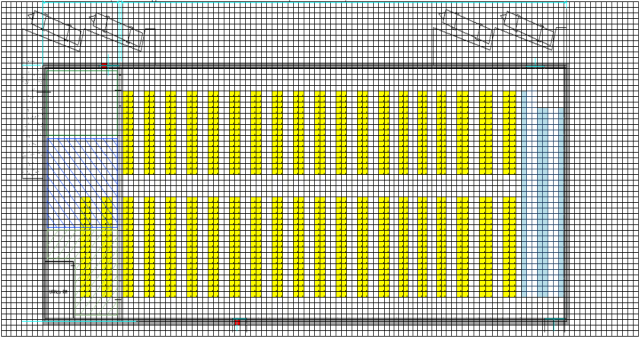
\includegraphics[width=0.99\linewidth]{figures/slap_ea/DesignTool.png}
    \caption{Na obrázku je možné vidět příklad jednoduchého nástroje pro tvorbu modelu skladu, a také v něm vytvořeného modelu skladu. Obrázek převzat z práce~\cite{slapSeacomp}.}
    \label{fig:slapDesignTool}
\end{figure}

Příklad toho, jak může vypadat takový nástroj pro vytvoření virtuálního modelu skladu lze vidět na obrázku~\ref{fig:slapDesignTool}. V závislosti na možnostech nástroje je uživatel schopen si sám jednoduše vytvořit virtuální reprezentaci svého existujícího skladu (měřítko vůči reálnému světu, pozice lokací a slotů, vstupů a výstupů skladu, či dopravníků propojující jednotlivé komponenty). Tato reprezentace může uživateli pomoct při rozhodování za pomoci zmíněných analýz.

\section{Simulace skladu}
Automatizované sklady jsou velmi komplexní systémy. Často mají mnohá omezení daná jejich layoutem, způsobem manipulace s produkty (dopravníky, vysokozdvižné vozíky, \ldots), úložnými a pickovacími politikami, a tak dále. Optimalizace výkonnosti takovýchto skladů často vyžaduje přesnou definici jejich modelu. Zmíněné praktiky jako ukládání či pickování produktů nelze jednoduše převést na matematické výrazy, které by šly optimalizovat standardním způsobem. Optimalizace takovýchto systémů je navíc často více-objektivní (např. co nejkratší doba pickovaní a zároveň co nejvyšší úspora místa), kdy se optimalizuje více parametrů zároveň a hledá se množina možných řešení která představuje kompromisy (ang. \emph{tradeoff}) mezi různými požadavky. Z toho vyplývá, že lepší způsob jak se vypořádat s řešením tohoto problému je pomocí programovacích technik, což de-facto znamená vytvořit simulátor skladu, odpovídající pokud možno co nejvíce reálnému modelovanému systému~\cite{whModelSim}.

Skladové systémy jsou vzhledem k jejich důležitosti v dodavatelském řetězci a potřebě optimalizace (resp. velké úspoře prostředků při jejich optimalizaci) velmi často předmětem simulování. V nejedné práci zabývající se problematikou SLAP se objevují nástroje pro simulaci skladu (příjem, pickování a odesílání objednávek, atp.). Tyto nástroje jsou nejčastěji založeny na diskrétních událostech. V posledních letech se však také objevují řešení založená na agentech. Simulace bývá zpravidla využívána za účelem sledování změn chování při použití různých strategií či konfigurací. Simulátor skladu byl využit například za účelem porovnání ujetých vzdáleností při použití různých strategií uložení produktů v automatizovaném prostředí skladu či vlivu použité alokace slotů na proces manuálního pickování objednávek~\cite{slapReview}.

Práce~\cite{whModelSim} definuje důležitost simulace skladu následujícími úkoly, jež dokáže plnit:

\begin{itemize}
    \item Poskytnutí tzv. \emph{proof-of-concept} (návrh konceptu).
    \item Analýza dopadů na potencionální změny v existujícím systému.
    \item Evaluace výkonnosti skladu již ve fázi návrhu, a to při různém zatížení.
    \item Optimalizace parametrů skladu (layout, úložné a pickovací politiky, \ldots).
    \item Analýza možných \uv{úzkých bodů} (ang. \emph{bottleneck}).
    \item Odhad neměřitelných proměnných a kvantit.
    \item Průzkum a testování nových skladových politik.
    \item Plánování kapacit skladu.
    \item Zodpovězení \emph{what-if} otázek (analýza).
\end{itemize}

Přístupy k simulaci skladu jsou tři. Buď lze využít existujících grafických aplikací, frameworků/knihoven či specializovaných programovacích jazyků. Grafické aplikace sice nevyžadují nutnost psaní kódu a vytvoření systémů je poměrně jednoduché, avšak jsou zpravidla velmi komplexní, drahé a nemusí poskytovat všechny potřebné funkcionality. Patří sem např. AutoMod\textsuperscript{TM} nebo Siemens Tecnomatix\textsuperscript{TM}. Softwarové knihovny poskytují programátorům před-připravené třídy a funkce, které jim pomohou k vytvoření vlastního simulátoru a jsou zpravidla založeny na simulaci diskrétními událostmi. Nevýhodou těchto knihoven je, že většina z nich je orientovaná na simulaci počítačových sítí a ve většině případů je nelze použít pro simulaci skladu (např. OMNeT++ a Ns2). V poslední řadě se používají specializované programovací jazyky mezi které patří např. SIMSCRIPT a SIMULA. Tyto jazyky ulehčují modelování problému pomocí sady před-připravených konstrukcí a instrukcí a jsou často zakomponovány v grafických aplikacích zmíněných výše. Mají však jistá omezení podobně jako softwarové knihovny~\cite{whModelSim}.

V této práci je využit druhý přístup a sice softwarová knihovna, která je zdarma k~použití, kompatibilní se zbytkem C++ programu a flexibilní.


\section{Související práce}
Současná odborná literatura zabývající se problematiku SLAP lze rozdělit do různých kategorií. Nejdůležitější jsou však dvě, a sice použitý přístup a optimalizovaná kritéria, viz~\ref{fig:grafPristupy}~a~\ref{fig:grafMeritka}. Tato práce kombinuje meta-heuristiku se simulací a optimalizovaným kritériem je čas zpracování sady objednávek. V tabulce \ref{tab:klasifikacePraci} lze vidět veškeré studované práce zabývající se problematikou SLAP klasifikované dle těchto kritérií~\cite{slapReview}.

\begin{table}[t]
\centering
\begin{tabular}{ll|l|l|l|l}
\toprule
 & & \multicolumn{4}{c}{\textbf{Použitá metoda}} \\

\multirow{ 7}{*}{\textbf{Optimaliz.}} & & Exaktní & Heuristická & Meta-heuristická & Simulace & \hline
   & Vzdálenost, prostor &  &  & \cite{slapGaMultiObj,optimisationOrderPickingGA} & \cite{whModelSim} &
   & Čas & \cite{slapSeacomp} & \cite{exactTimeSlap} &  &  &
   & Provozní efektivita &  &  & \cite{slapPickAndPass} &  &
\textbf{kritérium} & Náklady &  &  &  &  &
   & Lidské faktory &  &  &  &  &
   & Infrastruktura &  &  &  &  &
\bottomrule
\end{tabular}
\caption{Veškeré studované práce klasifikované podle použité metody a optimalizovaného kritéria. Práce by se daly klasifikovat na základě mnoha dalších kritérií, ale pro přehlednost byly zvoleny pouze dvě hlavní, a sice metoda a optimalizované kritérium.}
\label{tab:klasifikacePraci}
\end{table}


\begin{figure*}[t]
    \centering
    \begin{minipage}{0.49\textwidth}
        \centering
        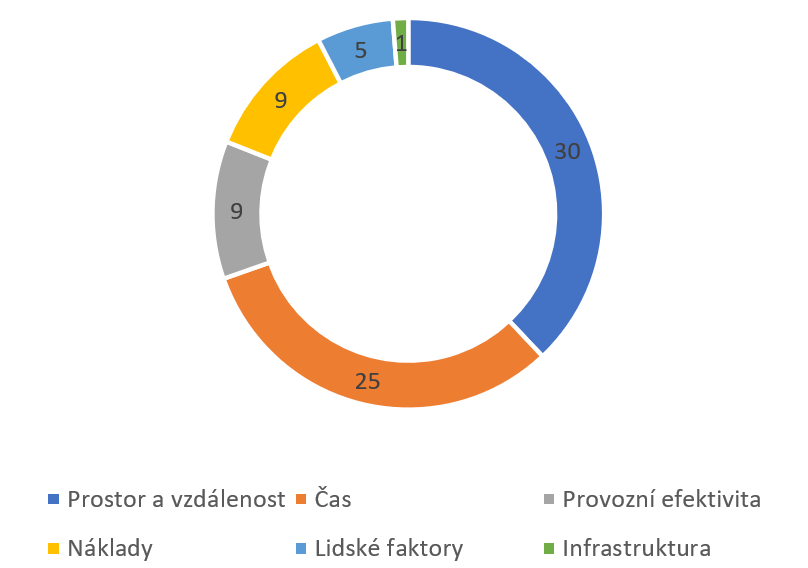
\includegraphics[width=1\textwidth]{figures/slap_ea/pristupyReseniSlapGraf.png}
        \caption{Graf udávající optimalizační kritéria pro řešení SLAP v odborné literatuře a jejich četnost. Vytvořeno na základě dat~z~\cite{slapReview}.}
        \label{fig:grafPristupy}
    \end{minipage}\hfill
    \begin{minipage}{0.49\textwidth}
        \centering
        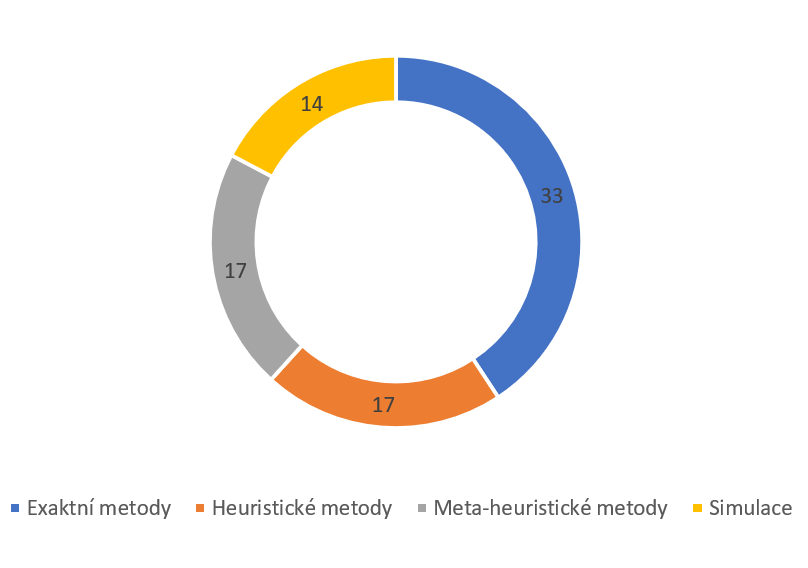
\includegraphics[width=1\textwidth]{figures/slap_ea/vykonnostniMeritkoGraf.png}
        \caption{Graf udávající optimalizované výkonnostní indikátory (KPI) skladu v odborné literatuře a jejich četnost. Vytvořeno na základě dat~z~\cite{slapReview}.}
        \label{fig:grafMeritka}
    \end{minipage}\hfill
\end{figure*}

V práci~\cite{slapSeacomp} autoři implementovali nástroj pro minimalizaci času zpracování objednávek. Práce řeší problém SLAP pomocí seřazení produktů od nejčastěji kupovaného po nejméně kupovaný a slotů lokací od nejbližšího k vchodu a východu ze skladu až po ten nejvzdálenější. Následně provádí namapování produktů do slotů tak, že nejčastěji kupovaný produkt je v nejvýhodnějším slotu, atd. Následně byl nástroj vyhodnocen na modelu existujícího skladu a bylo zjištěno, že časy manipulace s materiálem byly zredukovány o $37.8\%$ oproti původnímu stavu. Tento princip byl pro porovnání využit i~v~této práci a lze jej vidět v~grafu \ref{fig:vyhodnoceniGrafTrain} jako \texttt{Battista a spol}. Při experimentech v této práci dosáhl zlepšení $33.2\%$.

Genetický algoritmus pro minimalizaci ujeté vzdálenosti ve skladu byl použit v~práci~\cite{optimisationOrderPickingGA}. Autoři optimalizovali přesně definovaný model skladu daný zákazníkem popsaný matematickou funkcí, a podařilo se jim snížit cestovanou vzdálenost ve skladu při zpracovávání objednávek o $28\%$. To vede ke značnému zrychlení pickování.

Řešení problematiky SLAP pomocí meta-heuristického přístupu založeného na genetických algoritmech se objevilo také v práci~\cite{slapPickAndPass}. Byla zde vytvořena matematická objektivní funkce, která přesně popisovala rozložení skladu. V této práci autoři počítali také s doplňováním produktů a soustředili se na zjištění důležitosti rozložení zátěže mezi jednotlivé pickery, které je dle nich esenciální pro správnou optimalizaci.

Autoři práce~\cite{whModelSim} se kvůli složitosti a možnému zavedení chyb či ignorování přepisu skladu na matematickou funkci rozhodli využít pro vyhodnocení simulátor skladu. Autoři zmiňují, že ze všech možných kombinací druhů simulace skladu je nejvhodnější a nejpřirozenější simulace pomocí diskrétních událostí, protože sklad je v podstatě kolekce entit, které reagují na fixní události (jako je například pickování objednávek). Dále byla v rámci práce provedena případová studie existujícího skladu a implementován simulátor daného skladu. Výsledkem každé simulace byl soubor obsahující veškeré KPI skladu, které mohli být dále jednoduše použity pro srovnávání a podařilo značně zvýšit množství uložených produktů.

Heuristický přístup byl použit v práci \cite{exactTimeSlap}. Byl vytvořen komplexní matematický model skladu a pomocí celo-číselného programování byl optimalizován čas cesty po skladu. V práci byl implementován heuristický vyhledávací algoritmus tabu a pro malé problémy nalezl algoritmus vždy optimální řešení.

Podobně jako ve zmíněných pracích je i zde experimentováno se základním i genetickým přístupem. Navíc je práce doplněna i o jiné optimalizace a umožňuje uživateli nastavit si vlastní sklad a strukturu objednávek, všechno v rámci grafické aplikace.
